\section{Multiplikation und Division mit Brüchen}\vspace{-1em}
Bei der Berechnung von Bruchteilen von Größen in \autoref{sec:bruchteile} haben wir bereits Brüche mit natürlichen Zahlen multipliziert. Dabei wurde die natürliche Zahl immer mit dem Zähler multipliziert und durch den Nenner dividiert. Die Multiplikation mit einem Bruch verlangte also immer zwei Punktrechnungen, deren Reihenfolge frei gewählt werden konnte:
\begin{equation*}
	\frac{3}{4}\cdot 12 = (12\cdot3) : 4 = 36:4 = 9\text{ liefert das gleiche wie }\frac{3}{4}\cdot 12 = (12:4)\cdot 3 = 3\cdot 3=9
\end{equation*}

\subsection{Bruch mal Zahl}\vspace{-1em}
Weil in der Multiplikation vertauscht werden darf ($3\cdot4=4\cdot3$), ist es egal, ob wir den Fall $Bruch\cdot Zahl$ oder $Zahl\cdot Bruch$ betrachten. 

Bei der Rechnung $3\cdot \frac{7}{8}$ lässt sich die Division weder vor der Multiplikation ($3:8$) noch danach ($3\cdot7:8=21:8$) durchführen ohne, dass ein Rest entsteht. Wir können das Ergebnis aber dennoch angeben in der Bruchschreibweise
\begin{equation*}
	3\cdot \frac{7}{8} = \frac{3\cdot 7}{8}=\frac{21}{8}
\end{equation*}
Das gleiche Ergebnis erhalten wir auch, wenn wir die Multiplikation als mehrfaches Addieren umschreiben (hier drei mal $\frac{7}{8}$ mit sich selbst addieren):
\begin{equation*}
	3\cdot \frac{7}{8} = \frac{7}{8}+\frac{7}{8}+\frac{7}{8}=\frac{21}{8}
\end{equation*}

\COLBOX{
	Merke: Wenn man eine ganze Zahl mit einem Bruch multipliziert, muss man die ganze Zahl mit dem Zähler multiplizieren. Der Nenner bleibt gleich.
	\begin{equation*}
		Zahl\cdot Bruch = Zahl\cdot \frac{Z}{N}=\frac{Zahl\cdot Z}{N}
	\end{equation*}
}
Hinweis: Das Ergebnis kann evtl. noch gekürzt werden.

\subsubsection*{Übungen:}\vspace{-1em}
\begin{enumerate}[label=\alph*)]
	\item \RED{Übung Bruch mal Zahl}
\end{enumerate}

\subsection{Bruch durch Zahl}\vspace{-1em}
Werden Brüche durch Zahlen geteilt. Zum Beispiel teile $\frac{1}{2}$ durch $3$. Dann teilen wir den bestehenden Bruchteil in ebenso kleine Teile und nehmen einen davon. In \autoref{fig:half2third} ist dieser Vorgang für einen Kreis dargestellt. Im rechten Kreis entspricht der markierte Teil einem Sechstel des ganzen Kreises. Ebenso ist $\frac{1}{2}:3=\frac{1}{2\cdot 3}=\frac{1}{6}$.

\begin{figure}
	\centering
	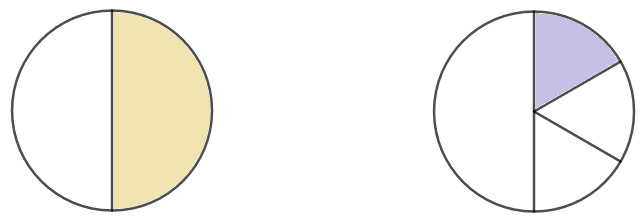
\includegraphics[width=0.7\linewidth]{fig/half2third}
	\caption[Halbes zu Drittel]{Links: Halber Kreis ist markiert. Rechts: Der halbe Kreis wurde in drei gleich große Teile zerlegt. Das markierte Teil ist ein Drittel des halben Kreises.}
	\label{fig:half2third}
\end{figure}


\COLBOX{
	Merke: Wenn man einen Bruch durch eine Zahl dividiert, muss man die ganze Zahl mit dem Nenner multiplizieren. Der Zähler bleibt gleich.
	\begin{equation*}
		Bruch: Zahl = \frac{Z}{N}:Zahl=\frac{Z}{Zahl\cdot N}
	\end{equation*}
}
Hinweis: Das Ergebnis kann evtl. noch gekürzt werden.

\subsubsection*{Übungen:}\vspace{-1em}
\begin{enumerate}[label=\alph*)]
	\item \RED{Übung Bruch durch Zahl}
\end{enumerate}

\subsection{Multiplikation von Bruch mit Bruch}
Die Multiplikation von einem Bruch mit einem anderen ist letztlich nichts anderes als eine Multiplikation des einen Bruches mit dem Zähler des zweiten und Division mit dessen Nenner. 

Nehmen wir mal wieder das Beispiel der dreiviertel Stunde und schauen, was $\frac{2}{3}$ einer $\frac{3}{4}h$ sind. So müssen wir die Dreiviertelstunde erst verdoppeln, weil der erste Bruch eine eine zwei im Zähler hat. Das Ergebnis dieser Rechnung wird anschließend durch drei dividiert, weil im Nenner des ersten Bruches eine drei Steht.
$$\frac{2}{3}\cdot \frac{3}{4}h=2\cdot \frac{3}{4}h:3= \frac{2\cdot 3}{4}h:3=\frac{6}{4}h:3=\frac{6}{4\cdot 3}h=\frac{6}{12}h\underset{6}{=}\frac{1}{2}h$$

Die gleiche Überlegung mit Umwandlung der dreiviertel Stunde in Minuten liefert:
$$\frac{2}{3}\text{ von }45min. = \frac{2}{3}\cdot 45min. = \frac{2\cdot 45}{3}min. = \frac{90}{3} min. \underset{3}{=}30min.=\frac{1}{2}h$$
Fasst man die beiden Schritte \emph{Multiplikation mit Zähler} und \emph{Division mit Nenner} zusammen werden die Brüche multipliziert, indem Zähler und Nenner des einen Bruches jeweils mit dem Zähler bzw. Nenner des anderen Bruches multipliziert werden.

\COLBOX{
	Die Multiplikation von Brüchen erfolgt nach dem Prinzip \glqq{}\emph{Zähler mal Zähler durch Nenner mal Nenner}\grqq{}:
	\begin{equation*}
		Bruch1\cdot Bruch2 = \frac{Z1}{N1}\cdot \frac{Z2}{N2} = \frac{Z1\cdot Z2}{N1\cdot N2}
	\end{equation*}
}

Bemerkung: Bei der Multiplikation von Brüchen berechnet man \emph{Anteile von Anteilen}.

Beispiel:
\begin{equation*} 
	\frac{3}{4}\text{ von }\frac{2}{5} = \frac{3}{4} \cdot \frac{2}{5}= \frac{3\cdot 2}{4\cdot 5}= \frac{6}{20}
\end{equation*}

\subsubsection*{Übungen:}\vspace{-1em}
Berechne (Lösungen in der Fußnote\footnote{a) $\frac{6}{35}$; b) $\frac{30}{44}=\frac{15}{22}$; c) $\frac{28}{40}=\frac{7}{10}$; d) $\frac{6}{72}=\frac{1}{12}$})
\begin{multicols}{4}
\begin{enumerate}[label=\alph*)]
	\item $\frac{3}{5} \cdot \frac{2}{7}$
	\item $\frac{10}{11} \cdot \frac{3}{4}$
	\item $\frac{7}{8} \cdot \frac{4}{5}$
	\item $\frac{1}{9} \cdot \frac{6}{8}$
\end{enumerate}
\end{multicols}

\subsection{Division von Bruch durch Bruch}\vspace{-1em}
Division wurde bislang immer durch die Frage \glqq{}Wie oft passt eine Zahl in eine andere Zahl?\grqq{} begleitet. 
Die Rechnung $12:4=3$ beantwortet z.B. die Frage: \glqq{}Wie oft passt die vier in die zwölf?\grqq{}.

Bei der Division mit ganzen Zahlen kam es mitunter vor, dass ein Rest übrig blieb. Durch Brüche können wir diesem Rest nun einen festen Wert geben. Die Rechnung 
$	13:4 = 3 R 1 $ wird so zu $13:4= 3+\frac{1}{4}$
Es passen also drei ganze und ein viertel von $4$ in die $13$. Das zeigt euch die klassische Probe per Gegenrechnung:
\begin{equation*}
	\left(3+\frac{1}{4}\right)\cdot 4 = 3\cdot 4 + \frac{1}{4}\cdot 4 = 12 + 1 = 13
\end{equation*}

Es können so beliebige Divisionen durchgeführt werden. Es kann dabei sogar passieren, dass der gefragte Teiler (Divisior) kein einziges Mal komplett in den Dividend passt, jedoch ein Bruchteil des Divisors.

Beispiel: Das ein viertel zwei mal in ein halbes passt, ist vermutlich leicht verständlich. Aber wie oft passt ein viertel in ein achtel?

Rechne: $\frac{1}{8}:\frac{1}{4}=\frac{1}{2}$. Es passt ein halbes viertel in ein achtel.

BILDER

\COLBOX{
	Brüche werden dividiert, indem mit dem Kehrwert des Divisors multipliziert wird. Der Kehrwert ist der Bruch mit vertauschtem Zähler und Nenner
	\begin{equation*}
		Bruch1: Bruch2 = \frac{Z1}{N1}: \frac{Z2}{N2} = \frac{Z1}{N1}\cdot \frac{N2}{Z2} =\frac{Z1\cdot N2}{N1\cdot Z2}
	\end{equation*}
}

Beispiel:
\begin{equation*}
	\frac{5}{12}:\frac{5}{6}= \frac{5}{12}\cdot \frac{6}{5}=\frac{5\cdot 6}{12\cdot 5}= \frac{30}{60}\underset{30}{=}\frac{1}{2}
\end{equation*}
Das bedeutet: Es passt ein halbes $\frac{5}{6}$-Stück in ein $\frac{5}{12}$-Stück.

mehr folgt später... \ {mehr multi div mit frac}

\subsubsection*{Übungen:}\vspace{-1em}
\begin{enumerate}[label=\alph*)]
	\item \RED{Übung Bruch durch Bruch}
\end{enumerate}